\documentclass{article} % For LaTeX2e
\usepackage{nips15submit_e,times}
\usepackage{hyperref}
\usepackage{url}
\usepackage{graphicx}
\usepackage{bbm}
\usepackage{amsmath}
\usepackage[psamsfonts]{amssymb}
\graphicspath{ {images/} }
\usepackage{algorithm}
\usepackage{algorithmic}
\usepackage[square,numbers]{natbib}

\bibliographystyle{unsrtnat}

%\documentstyle[nips14submit_09,times,art10]{article} % For LaTeX 2.09
\title{Multi-region demixing of brain transcriptome}
% \addbibresource{nmf_multi.bib}

\author{
Lior Kirsch \\ Bar Ilan university \\ Ramat Gan 52900 Israel \\ 
\And
Gal Chechik \\ Bar Ilan university \\ Ramat Gan 52900 Israel \\
\texttt{gal.chechik@biu.ac.il} \\
}
\newcommand{\fix}{\marginpar{FIX}}
\newcommand{\new}{\marginpar{NEW}}
\newcommand{\reals}{\mathbb{R}}
\newcommand{\W}{W}
\renewcommand{\eqref}[1]{Eq.~(\ref{#1})}
\newcommand{\figref}[1]{Fig.~(\ref{#1})}
\newcommand{\figureref}[1]{Figure~(\ref{#1})}
%\nipsfinalcopy % Uncomment for camera-ready version
\begin{document}
\maketitle
\begin{abstract}
    High quality and large scale measurements of gene expression in the brain have been collected across many species, many regions and many ages, but unfortunately, almost all these measurements reflect  expression of an uncontrolled mix from various cell types including neurons, glia and blood cells. This fact hinders the insights that can be gained by analyzing datasets of gene expression in the brain. Inferring cell-type specific information from these mixtures is a key challenge. We propose here a probabilistic approach to blindly demix brain transcriptome samples, building on variability of cell-type proportions across samples. We further describe a model that takes into account that tissues in different brain structures differ in their expression profiles by introducing soft-sharing between cell-type-specific profiles from different brain regions. We describe an efficient algorithm to estimate the parameters of the model, as well as techniques to determine some of its hyper parameters from prior knowledge. We study the regimes where multi-region demixing works well using controlled data and evaluate the approach using RNA-seq profiles measured from multiple regions in postmortem human brains. Predictions are validated against ground-truth data of cell-type specific profiles measured in corresponding regions in the mouse brain, showing that soft demixing successfully outperforms baselines of demixing unified and individual regions. 
\end{abstract}

\section{Introduction}
\label{introduction}
Recent advances in molecular biology techniques allow to measure transcriptome profiles across the brain at unprecedented quality and magnitude. Large datasets of gene expression in the brain are now available, covering  many brain regions, ages and species. RNA sequencing techniques now provides accurate genome-wide counts of transcripts for each gene and splice variant. Unfortunately however, when gene expression is measured in a complex tissue, like the brain, the measured transcripts reflect an uncontrolled mix of expression from multiple cell types including neurons, astrocytes, oligodendrocytes and even blood and immune system cells. This limits the analysis and understanding that can be gained from gene expression measurements of the brain. Although several techniques have been developed to isolate and purify cells of individual types and measure their transcription profiles \cite{okaty2011cell,barres2014,darmanis2015survey}, these techniques are costly and complex, and only a handful of cell-type isolated profiles have been collected so far. 

The current paper proposes a computational technique to demix gene expression measurements in the brain. The idea is simple: when multiple samples are collected from the brain, their cellular composition often varies slightly from one sample to another. Each sample therefore reflects mixtures with different proportions of cell types. We propose here to model transcriptome profiles as a mixture of contributions from different cell types, and describe how the latent component that are shared across samples can be found.

Developing robust methods to extract cell-type specific signals from transcriptome mixtures, has a potential to be extremely useful. It could provide deeper analysis of data that was already collected and is very hard and costly to reproduce. For example, collecting brain banks in human patients with brain disorders is a complex and lengthy process, so extracting cell-type level information from existing brain transcript datasets can help delineating the role of neurons and glia in diseased like Alzheimer (AD) or Epilepsy.

In the mouse brain, a demixing approach was recently applied to ISH transcriptome measures \cite{grange2014cell}, where expression profiles were demixed using known cell-type-specific profiles. Here we take a further step and apply blind demixing, inferring both the mixture components and their proportions. We use isolated cell-type profiles for validation but not during training. 

%Demixing transcriptome profiles into their components has been applied in various domains outside neuroscience \cite{}.

Importantly, collections of transcriptome measurements in the brain have a unique structure that we suggest to benefit from. In the brain, gene expression profile changes from one brain region to the other, in a way that often follows the developmental hierarchy of brain regions \cite{zapala2005}. This suggests that we can use a-priori knowledge about regions which are expected to share similar expression profiles. For instance, pyramidal cells can be found in most neocortex areas, hence may express a highly preserved set of genes. At the same time, neurons in the hippocampus (an archeo-cortical region) may exhibit an expression profile that is less similar to the neocortical profile. Figure 1 shows a hierarchy of brain regions based on embryonic development developed by the Allen brain institute. 

\begin{figure}[!hbt]
  \begin{minipage}[c]{0.65\textwidth}
    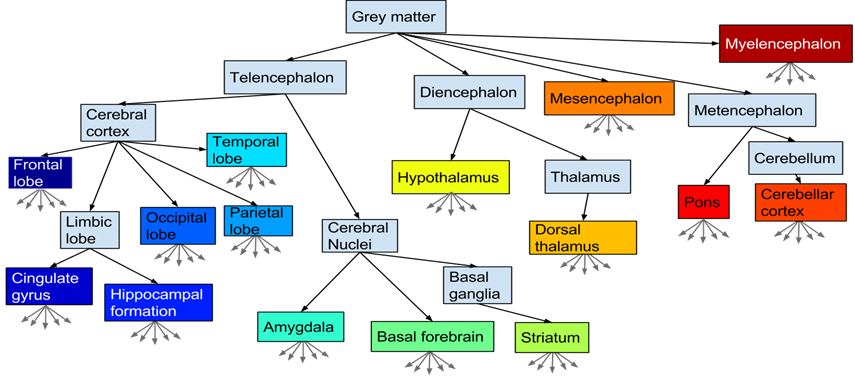
\includegraphics[width=\textwidth]{tree}
  \end{minipage}\hfill
  \begin{minipage}[c]{0.3\textwidth}
    \caption{Hierarchical relations among brain regions. An ontology of regions of the human brain has been created based on neural development. Colored boxes correspond to brain regions that we analyzed below. The color scheme is based on caudal-rostral axis of brain regions, from red hindbrain to blue forebrain.} 
    \label{fig:bro}
  \end{minipage}
\end{figure}

This hierarchical structure suggests that when applying demixing to brain-omics data, one should be careful not to treat all brain samples as homogeneously containing the same set of neurons and underlying expressed genes. Instead, we can take into account the relative similarity among brain structures. 

To combine the various sources of prior information, our approach is based on a probabilistic model with three components. First, a set of samples from a single brain region is represented as a mixture of a smaller number of components. Second, we can include a prior on each of these underlying cell-type-specific profiles based on previous measurements. Third, we add pairwise attractive potentials, pushing expression profiles of related regions to be similar.
 
This paper makes three main novel contributions. First, it describes for the first time blind demixing and multi-region demixing of transcriptome measurements. Second, it characterizes the regime of parameters where blind demixing works best in controlled mixtures. Finally, it demonstrates that demixing can uncover latent factors in RNA-seq measurements from multiple human brain regions.
 
The paper is organized as follows: We start by describing a probabilistic model of expression mix in a single region and and multiple regions. We then describe algorithms to optimize the parameters of the these model. Section 5, evaluate the regime of parameters where the demixing algorithm works well using we a controlled mix dataset that we created. Section 6 evaluates the algorithms in expression dataset from postmortem human brains.

% ==========================================
\section{A probabilistic model for multi-region demixing}

\newcommand{\x}{\mathbf{x}}
\renewcommand{\c}{\mathbf{h}}
\renewcommand{\H}{{H}}
\newcommand{\Htext}{{C}}
\newcommand{\paren}[1]{\left({#1}\right)}
\newcommand{\brackets}[1]{\left[{#1}\right]}
\newcommand{\norm}[1]{\|{#1}\|}
\newcommand{\argmin}{\operatornamewithlimits{argmin}}.

Our probabilistic model assumes that samples taken from the same brain region share common underlying factors, each factor reflecting the expression profile of an isolated cell type. The model also assumes that the expression profiles of different brain regions are similar but not identical, and therefore we aim to jointly learn all cell-type profiles of all regions. We start by describing a  probabilistic mixture model for samples from a \em{single} brain region, which we extend to the \em{multi-region} case in section 2.2.

\subsection{Model of a single brain region}
% ---------------------------------
Let $\{\x_1, \ldots, \x_n\} \in \reals^d$ be a set of samples. Our model assumes that each sample $\x_i$ is obtained from a noisy mixture of $K$ cell types, each having its own {\em {hidden profile}} $\{\c_1, \ldots \c_K \}\in \reals^d$.

We model each sample $x_i$ as a noisy mixture
\begin{equation*}
 \x_i = \sum_{k=1}^K p_{ik} \c_k + \xi_i \quad\forall i \quad,
\end{equation*}
where $p_{ik}$ is the proportion of the cell type $k$ in the sample $i$, $\sum_k p_{ik} = 1, \forall i$, and $\xi_i \sim N(0,\sigma^2)$ is additive Gaussian noise independent at each sample. We further assume a Gaussian prior distribution $p_0( \c_1, \ldots, \c_K)$ over each cell type $ \c_k  \sim N(\mu_k, \Sigma) $, and over the mixture proportions $p_0(p_1, \ldots p_K)$. The parameters $\mu_k$ and $\Sigma$ can be estimated in advance from available measurements of expression in isolated cell types \cite{okaty2011cell,darmanis2015survey}.

Together, the probability of an observed sample $x_i$ is
\begin{equation*}
    P(\x_1,\ldots,\x_n | \{\c_k\}, \{p_{ik}\}) =  \frac{1}{\sqrt{2\pi}\sigma} \exp\left(-\frac{1}{2\sigma} (x_i - \sum_{k=1}^K p_{ik} \c_k)^2 \right)
\end{equation*}
and the minus log posterior of all the data equals (up to linear constants)
\begin{equation*}
    - log P(\x_1,\ldots,\x_n, \H, P| \mu, \Sigma) \propto
    \sum_{i=1}^n \paren{ \frac{1}{\sigma} (x_i - \sum_{k=1}^K p_{ik} \c_k)^2 }
     + \sum_{k=1}^K (c_k-\mu_k)^T\Sigma^{-1}(c_k-\mu_k)
\end{equation*}

Using matrix notation, we denote by $\H$ the $K \times d$ matrix of hidden profiles per cell type whose columns are $\brackets{\c_1, \ldots, \c_K}$; we denote by $W$ the $n \times K$ matrix of proportions $p_{ik}$,
and by $X$ the matrix whose columns are the samples $\brackets{\x_1,..., \x_n}$. This yields that maximizing the log posterior is equivalent to minimizing 
\begin{equation}
    \label{eq-single}
    \begin{aligned}
        & \underset{\cal{\H},\cal{W}}{\text{min}}  
        & & \norm{X - W \H}_F^2 + \sigma \norm{ \H - M }^2_{(\Sigma^{-1})}\\
            & \text{subject to} &
            & W^r_{l,j} \geq 0 \;\; \forall j, l, \\
        & & & H^r_{j,d} \geq 0 \;\;\forall j, d \\
        & & & \sum_j W^i_{l,j} = 1 \;\; \forall l \\
        \end{aligned}
\end{equation}
where $\norm{\cdot}_F$ is the Frobenius norm, $M$ is a matrix whose columns are the expected cell-type profiles $\mu_k$ and  $\|\cdot\|_{\Sigma}$ is the norm through a PSD matrix $\Sigma$. The constraints on $\W$ are because the elements in each row of $\W$ are mixture probabilities. The constraints on $\H$ are because the elements of $\H$ are counts of expressed transcripts.

\subsection{Multiple regions}
%-------------------------------
We now turn to extend single-region demixing to handle demixing of samples collected from several brain regions. 
As far as we are aware, this is the first probabilistic model for demixing multiple sets of samples.

We assume that expression profiles of an each cell type can vary from one region to another, but is likely to remain similar. The strength of similarity between the expression profiles in two regions depends on how closely related two brain regions are. For instance, neurons in cortical regions may be very similar to each other, less similar to the hippocampal neurons and far less similar to the cerebellar neurons. 

To capture these relations our model introduces pair-wise attractive potentials between the cell-type profile in one region $\c^r_k$ to the profile of the same cell type in another region $\c^s_k$. The strength of the attraction depends on the relatedness $\phi_{r,s}$ of two brain regions, and on a global hyper parameter that controls the relative weight of edge potentials compared with node potentials. Together, this yields pairwise potential terms of the form 
$\lambda \phi_{r,s}|| \c^r_k - \c^s_k||^2$.

This soft-sharing approach can be seen as a balance between two extremes. At one extreme (no pairwise attraction, $\lambda=0$), demixing of each regions is trained independently. With current datasets, this approach usually has too few samples per regions.  At the other extreme (strong pairwise attraction, $\lambda \gg 0$), one could treat all samples as being created from a single set of underlying latent factors, as if all brain regions share a single expression profiles per cell-type. In this case, more samples are available for estimating the (fewer) latent factors, but the wrong assumes that expression is homogeneous across the brain   distorts the resulting profiles. Our soft-sharing approach bridges the two extremes by controlling how profiles of different regions share common traits. Similar soft sharing has often been used in supervised multi-task learning (MTL). 

Formally, given sets of samples from $R$ regions ${\cal{X}} = \{X^1,\ldots, X^R\}$, where $X^r = \{\x^r_1, \ldots, \x^r_{n_r} \}$, we learn $R$ sets of hidden cell-type-specific profiles ${\cal{\H}} = \{\H^1,\ldots, \H^R\}$ and their corresponding proportions ${\cal{W}} = \{ W^1,\ldots W^R\}$. Adding Gaussian potentials over cell-type profiles from a pair of regions ($\H^r$, $\H^s$) with a weight of $\lambda_{r,s}$ amounts to a quadratic term in the log posterior. This therefore yields the following optimization problem
\begin{equation}
    \label{eq-multi}
    \begin{aligned}
        & \underset{\cal{\H},\cal{W}}{\text{min}}  
        & & \sum_{r=1}^R  \| X^r - W^r \H^r \|_F^2
        + \sum_{r=1}^R  \sigma^r \| M^r - \H^r \|^2_{(\Sigma^{-1})}  
        + \sum_{r \neq s} \lambda \phi_{r , s} \| \H^r - \H^s \|_F^2  \\
        & \text{subject to} &
            & W^r_{l,j} \geq 0 \;\; \forall j, l, r\\
        & & & H^r_{j,d} \geq 0 \;\;\forall j, d, r \\
        & & & \sum_j W^r_{l,j} = 1 \;\; \forall l,r \;. 
    \end{aligned}
\end{equation}
Once again the constraints on $\W$ are since these are the mixture proportions, and the constraints on all $\H$ reflecrt the fact that $\H$ holds counts of transcripts.

The proposed model is interestingly related to Markov random fields (MRFs). Consider a case where the mixture proportions $\cal{W}$ are given, then the probabilistic model over $\cal{\H}$ can be viewed as an MRF, where nodes correspond to the profiles of individual cell types across all regions $\c^1_1,\ldots, \c^r_k, \ldots \c^R_K$, node potentials reflect the priors $p_0(\c_k)$ based on known expression of individual cell types at various regions, and edge potentials reflect region-to-region similarity terms $\lambda \phi_{r,s}|| \c^r_k - \c^s_k||^2$. 

The next section discusses the algorithms we use to optimize this objective.

\section{Optimization}
% =====================
We now describe algorithms for optimizing the multi-region problem of \eqref{eq-multi}. We start with reviewing existing approaches for single-region demixing and then discuss multi-region demixing. 


% Our problem is well suited for performing block coordinate descent, both on the profiles and proportion matrices and both on the regions. At each iteration, we update the set of coordinates of a single region and freeze the coordinate of the rest of the region. After we update the profile matrices $H_n$ we proceed to update its proportion matrix $W_n$. Then, we cycle through the rest of the region and repeat until we converge. 

\subsection{Single-region demixing}
The demixing problem of \eqref{eq-single} is separately convex in $\H$ and $\W$ (quadratic objective with linear constraints), but not jointly convex in both. When the prior is discarded, it becomes equivalent to non-negative matrix factorization (NMF) \cite{leenmfs}, which has been intensively studied. Several approaches have been proposed to minimize the NMF objective.
%
% For the convergence I think we can claim something similar to:
% http://bioinformatics.oxfordjournals.org/content/23/12/1495.full
% In the section:
% Convergence properties of sparse NMF algorithms
% http://www.sciencedirect.com/science/article/pii/S0167637799000747#
Here we tested four methods: Multiplicative updates (MU) \cite{leenmfs}, and three variants of alternative least square (ALS) \cite{lin2007projected,kim2008activeset,kim2011fast}. 

{\bf {Multiplicative updates (MU)}}. Lee and Seung \cite{leenmfs} described an NMF algorithm based on multiplicative updates of W and \Htext. At each step, each coordinate of \Htext (and \W) is multiplied by a non-negative scalar, which gaurantees that non-negativity is maintained: $H_{qj} \leftarrow H_{qj} \frac{(W^TX)_{qj}}{((W^TW)H)_{qj}} \quad
\forall 1\leq q \leq k, 1\leq j \leq n$ and $W_{iq} \leftarrow W_{iq} \frac{(XH^T)_{iq}}{(W(HH^T))_{iq}} \quad \forall 1\leq i \leq m, 1\leq q \leq k$.
This procedure is guaranteed to converge \cite{leenmfs,lin2007convergence}. 
% They showed the objective after these updates is %non-increasing. Although in practice the %muliplcative-update method works well, it was suggest %by Gonzalez and Yin Zhang %\cite{gonzalez2005accelerating}  that the %non-increasing updates may not converge to a %stationary point within realistic time.

{\bf{Alternating least squares} (ALS)} A second set of approaches to minimize the NMF objective is based on the fact that the optimization problem in \eqref{eq-single} is convex in each of the variables \W (or \Htext), hence one can iterate between efficiently updating $\W$ and updating $\H$. This approach can be viewed as a block-coordinate minimization approach. In ALS, the two matrices are  repeatedly updated using $ W^{t+1} = \argmin_{W \geq 0 } f(W^t, H^t)$ and $H^{t+1} = \argmin_{H \geq 0 } f(W^{t+1},H^t)$. Several different method of solving non negative least squares (NNLS) have been proposed some especially tuned for NMF. \citet{lin2007projected} proposed projected gradient decent with step that is chosen using the Armijo rule. 
Kim and park \cite{kim2008activeset,kim2011fast} use an active set method to solve NNLS. They group their variables to an active set and a passive set and 
exchange variables between the two to find the optimal sets. Variables are added to the passive set (the set of strictly positive variables) if they improve the score. Notice that if the passive set was known in advance, then an NNLS problem is a simple unconstrained least squares. Another variant of this concept is done by the "the block pivoting method" which allows to change multiple variable between groups per iteration (as appose to a single variable using the active set method) \cite{kim2011fast}. {\bf{THE ALS SECTION SHOULD BE MUCH SHORTER}}

In \eqref{eq-single} the rows of $\W$ are constrained to sum to one. This constraint is often relaxed during optimization. In practice, it is often replaced with a simple heuristic of normalizing each row of W after the optimization is completed. 

The above discussion focused on the first term in \eqref{eq-single}, omitting the prior term. Using the fact that we alternate between $\W$ and $\H$ the priors can be elegantly added by a simple transformation. Each time before we solve the minimization problem for H we perform:
$ X_{priors} = \Big[ X ;\Sigma^{-\frac{1}{2}} \Big]  $  ,  $ \W_{priors} = \Big[  \W ; \Sigma^{-\frac{1}{2}} M \Big]  $. We then find the minimum for $H$ using $X_{priors} $ and $W_{priors} $. 



\subsection{Multi-region demixing}
% ----------------------------------
The multi-region demixing model of \eqref{eq-multi} defines a jount optimization problem over all cell-type profiles $\cal{\H}$ and their proportions across all regions $\cal{\W}$.

Given values for the hyper parameters $\lambda$, $\sigma^r$ and $\phi_{r,s}$, 
we optimize \eqref{eq-multi} by extending the alternating least square (ALS) approach, this time solving separately for ${\H^r}$ and ${\W^r}$ of each region given all the other regions. This approach has similar convergence guarantees as the original ALS approach.  {\bf{ LIOR CAN YOU SPECIFY? AND ADD A REF}}

We initialize $\W^r$ with values in the range [0,1] and initialize $\H^r$ by random data samples with multiplicative noise. In practice, we found that it helped to start optimization by solving for each region separately, alternating over $\H$ and $\W$ for that region. We believe that this helped the profiles to more easily reconstruct their own unique profile. This 'warm-start' was then used to initialize the global ALS optimization. 
% We have also experimented with a few method to enforce the constrains on the proportion matrix. while some s%%Then prior to starting the loop, we warm initialize the profiles by performing a single step of block coordinate decent for each ($H^r,W^r$).

The values of the hyper parameters $\lambda$ and $\sigma^r$ can be found using cross validation. However, searching over all pairwise weights $\phi_{r,s}$ maybe prohibitive. We therefore used prior knowledge to determine the values of $\phi_{r,s}$. The strength of these hyper parameters reflects our prior belief on how strongly cell-type specific expression should be similar in two given regions, like the the expected similarity of a cortical to a hippocampal neuron.
To determine the values of $\phi_{r,s}$, we used a brain region hierarchy developed by the Allen institute of brain research (\figref{fig:bro}) to compute the tree-depth of the closest common ancestor of two brain regions $r$ and $s$. We used this depth as an estimate of $\log(\phi_{r,s})$. For example, the cerebellum and the occipital lobe  in this hierarchy are joined only at the root so we set their $\phi_{cerebellum, occipital} = \exp(1)$. 
%Specifically, at stage $t+1$ we update the profile matrix of %region r$ \H_r^{t+1} $ using the related profiles as priors.
%For the regularize parameters we use a base $\lambda$ times a distance factor between pairs of regions. 

Algorithm (1) desribes our training procedure.

\begin{algorithm}[tbh]
   \caption{Multi-region demixing}
   \label{alg:multimix}
   \begin{algorithmic}[1]
   \STATE {\bfseries input:} training data $X$, number of steps, $\lambda$, $\{\sigma^r\}$, $\{\phi_{r,s}\}$, $\{\mu^r_k\}$, $\Sigma$
   \STATE {\bfseries initialize:} for every region $r$
   \STATE \quad Initialize $\W^r$ and $\H^r$ with random values.
   %\REPEAT
   \STATE {\bfseries warm-start:} for every region $r$ 
   \STATE \quad Find optimal $\W^r$ and $\H^r$ for the single-region objective \eqref{eq-single}
   \STATE \quad $H^r = \argmin_{H \geq 0 } \| X^r - W^rH\|^2_F +  \sigma^r \| M^r - \H \|^2_{(\Sigma^{-1})} $
   \STATE \quad $ W^r = \argmin_{W \geq 0} \| X^r - WH^r\|^2_F $
   \REPEAT
   \STATE Select a region $r$ from a predefined random permutation.
   \STATE Find optimal $\W^r$ and $\H^r$ for the multi-region objective \eqref{eq-multi} using the rest of the regions as priors.
   \STATE  $H^r = \argmin_{H \geq 0 } \| X^r - W^rH\|^2_F + \sum_{r \neq s} \lambda \phi_{r , s} \| \H - \H^s \|_F^2  + \sigma^r \| M^r - \H \|^2_{(\Sigma^{-1})} $
   \STATE  $ W^r = \argmin_{W \geq 0} \| X^r - WH^r\|^2_F $
   \UNTIL{stopping condition}
\end{algorithmic}
\end{algorithm}




% ==========================================
\section{Related methods}
Demixing of transcriptome measurements into cell-type specific profiles has been mostly applied when a set of ground-truth underlying factors is known. \citet{shen2010cell} described demixing of 
whole-blood gene expression datasets from kidney transplants. \citet{grange2014cell} used isolated profiles of neurons and glia \cite{okaty2011cell} to map cell-type proportions across ISH measures of the mouse brain. Cell type demixing is also widely used in the context of immunology studies \cite{shen2013computational}.

Joint non negative matrix factorization of several matrices has been previously studied by \citet{lee2009group}. Their formulation introduced  both attractive and repulsive pairwise potentials, optimized using multiplicative updates. A Bayesian group factorization model was presented in \citet{shin2012bayesian}. Somewhat related, is the work by \citet{wang2012group}, who studied matrix factorization where some factors are shared across matrices.



% ==========================================
\section{Controlled experiments}
\label{Synthetic_exp}

With the goal of finding the regime of hyper parameters and optimization techniques where multi-region demixing works best , we start with a series of experiment where we mixed known expression profiles in a controlled way. This allowed us to solve mulit-region demixing in a settings where the latent factors are known and used as a ground truth. We first describe how the dataset was created and then characterize how performance depends on the number of samples and the number of latent factors (cell types).

\subsubsection*{Creating the mixture dataset}
We created controlled mixtures from a set of real transcriptome measurements, measured using microarrays from isolated cells. \citet{okaty2011cell} have collected 195 cell-type-specific profiles from 64 cell types spanning multiple regions and layers of the mouse brain. These profiles were previously measured after isolating cell using varous tehcniques (FACS, LMD).
 
Specifically, we create the known latent factors by collecting profiles for the 3 major population of cell types in the brain: neurons, astrocytes and oligodendrocytes. Each profile $\c$ is represented by 14580 genes. Profiles were extracted from 7 brain regions:  cortex layer 5A, cortex layer 5B, cortex layer 6, striatum, cerebellum, brainstem and the spinal cord. For each of these region, we also found the proportions of the three cell types reported in the literature \cite{Herculano2014}. (cortex:  0.7,0.1,0.2 for neuron, astrocytes, oligodendrocytes; cerebellum: 0.5,0.15,0.35, other: 0.65,0.1,0.25).

To draw a mixture sample, we drew proportion values $p_{neuron},p_{astro},p_{oligo}$ by adding multiplicative noise to the literature proportions. Each proportion was multiplied by a random value in [0,1] and scaled back to a  sum of 1. Finally, we added multiplicative Gaussian noise to the expression level of all genes, of the form $N(1,\xi^2)$, with noise levels of $\xi=10\%$ and $\xi=1\% $.

We then used the known mixtures to test the quality of reconstructed profiles as a function of number of samples, noise level, number of factors, and the optimization algorithm. 



%We evaluated the reconstructed profiles by computing their %spearman correlation with the true profiles. We then, %matched the best true profiles to the reconstructed %profiles.

%Each time we sampled n noisy samples and reconstructed the %profiles using these samples. The error bars in figure  %represented the sem over 30 repetitions.  

% \subsubsection*{bench-marking optimization method for single region NMF}

Since NMF is a non-convex problem different optimization techniques often reach different local minimas even when initialized using the same starting points. These differences in performance can result from the method of choice for each iteration (MM or ALS) or from the stopping and convergence rates of each alteration (in the ALS). We benchmarked 4 optimization techniques on data taken from a single region and found that all performed better with more samples. When the number of sample is sufficiently large we did not observe much difference in the performance of the different methods. while in a small number of samples the block-pivoting and the active-set performed slightly better (both had the same level of performance, and their graph overlaps) Figure \ref{fig:controlled_exp}(a).

%\subsubsection*{analyzing number of samples}
Next, we applied our multi-region demix to the controlled data from the 7 brain regions.
In the regime where only limited samples are available, there is sweet spot where we improve over the naive cases by using the connection between regions. As we increase the number of samples the benefit that we gain by using our method diminishes Figure \ref{fig:controlled_exp}(b). With enough samples solving the individual problems performs almost just as well. 


\begin{figure}[!hbt]
   (a) \hspace{120pt}(b) \hspace{120pt}(c) \hspace{120pt}
   \centering
     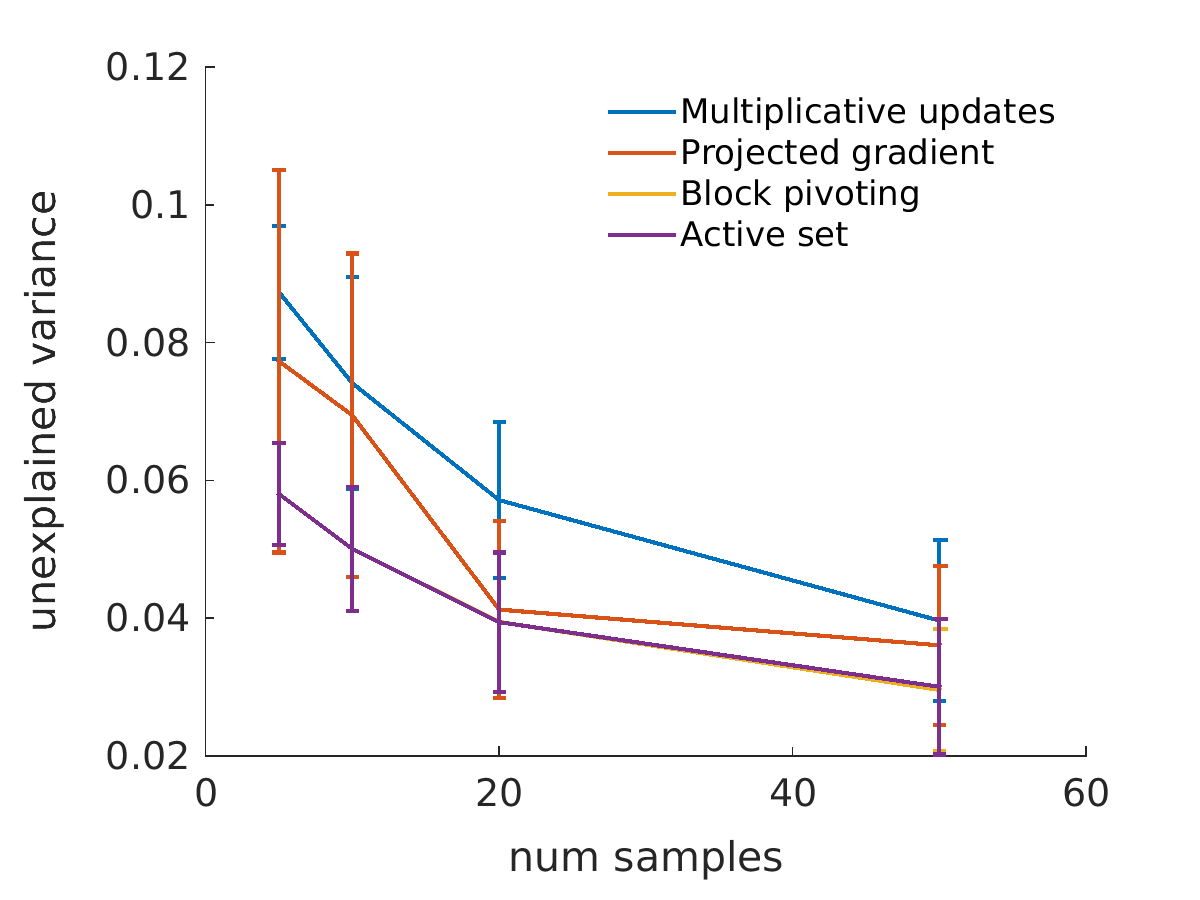
\includegraphics[width=0.32\textwidth]{methods}
     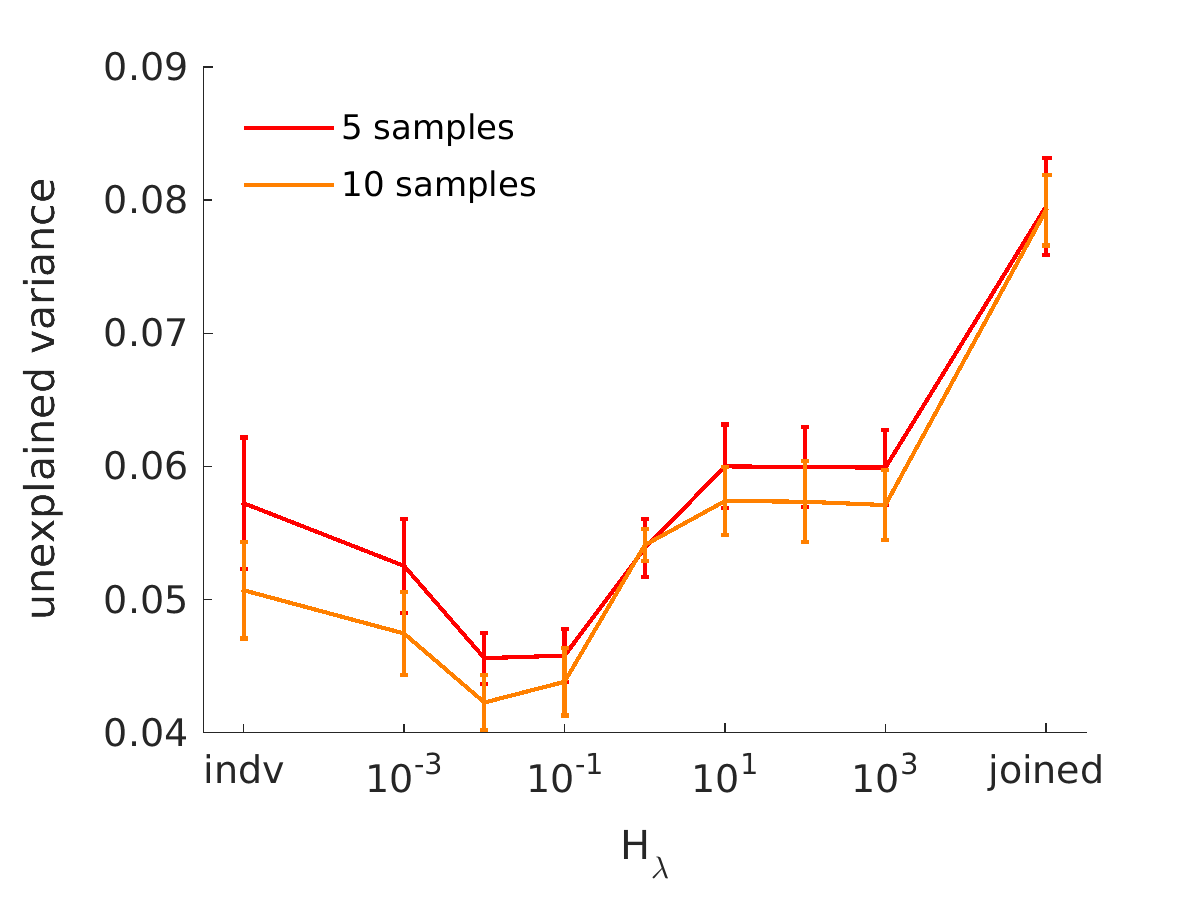
\includegraphics[width=0.32\textwidth]{lambda_samples}
     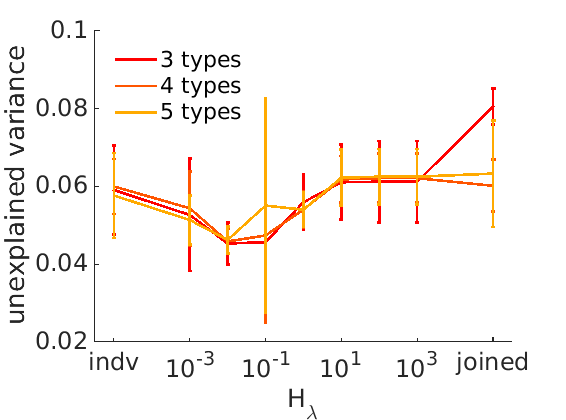
\includegraphics[width=0.32\textwidth]{num_types}
    \caption{Demixing in controlled experiments. 
    {\bf{(a)}}  Within a single region, all optimization methods improve when using more samples. The {\em active set} approach and the {\em block pivoting} outperformed other methods, particularly with few samples. {\bf{(b)}} Soft-sharing of latent factors lead to improved reconstruction in the multi-region settings, particularly with few samples. {\bf{(c)}} Reconstruction using more cell types then needed does not improve the results.} 
    \label{fig:controlled_exp}
\end{figure}

{\bf{LIOR, HOW MANY REGIONS IN FIGURE 2B?        - 7, I mentioned this above, in the creation of the dataset, is there anyplace you want to mention this again ?}}

%\subsubsection*{analyzing number of cell types}

As we increase the number of types the we are able to numerically better reconstruct the data matrix because we are allowing an approximation with of a larger rank. After we perform the demixing we match the best demixed profiles with true profile. This can improve the score since we can overfit. However, we did not notice any gain by using the extra profiles. It seems like it recovered the original profiles and some other vectors which helped to lower the overall fit but not the correlation to the original profiles. Overall it seems that this coincide with Ockham's razor and we can select simplest model which still capture the data \ref{fig:controlled_exp}(c). 


We found that the use of priors was somewhat fragile. While prior that were taken from the same experiment helped to imporve the score, priors of the same cell type just gathered in different experiments lowered our demixing success. 


% ==========================================
\section{Experiments with postmortem human brain expression}
\label{Human_exp}

We turn to analyze real mixtures collected using RNA-seq measurements from postmortem human brains. We used data from brainspan \cite{brainspan} (\url{http://www.brainspan.org/} and limited analysis to donors older than 17 years, leaving 8 adult human donors. We therefore had eight samples from each brain region. Each expression profile is represented by a vector of 52376 measurements including transcripts counts for coding and non-coding sequences. 

%Collecting human brain measurements is not easy to task since the the tissues has to be extracted not long after the subject death. So while the expression in each tissue can be represented in more details with the advancement of the sequencing tools, the number of samples is still extremely limited. For example, in our dataset there only few dozen samples and each is representation by tens of thousands features.

RNA sequencing is becoming the main way to measure gene expression in tissues, replacing the older microarrays technology. RNA sequencing provides more quantitative measurement since it actually counts the number of RNA transcripts in a tissue, as opposed to the more qualitative microarrays measurements. As such, RNA-seq data is more suitable for demixing since the number of RNAs transcripts grows linearly with the proportion of correspondiong cells in the tissue.

To evaluate the quality of demixing, we compare the inferred hidden cell-type specific profiles to transcriptome profiles measured in population of cells sorted by their cell type. At the time we conducted the analysis the cell-type specific RNA-seq data were only available in mouse \cite{barres2014}. We mapped the genes in the human to their orthologs in mouse and computed the spearman correlation between the reconstructed profiles and each of the single cell profiles. Recently such cell-type-specific data was made available for human, which will allow us to perform better validations. 

We determined the strengths of region-to-region relatedness $\phi_{r,s}$ based on the brain-region-ontology described in Figure \ref{fig:bro}. To verify that the human transcriptome measurements agree with this ontology, we first used an agglomerate hierarchical clustering over regions, by clustering expression profiles of these regions collected using microarray data by \cite{kang2011spatio}. The resulting region hierarchy had very string agreement with the brain region ontology, consistent with previous reports that adult expression patterns reflect brain development \cite{zapala2005}. The strengths of region-to-region attractive potentials $\lambda_{r,s}$ was determined as $\lambda \phi_{r,s}$ where $\lambda$ is a hyper parameter controlling the overall weight of edge potentials. 


Figure 3 shows the residual variance computed based on a Spearman correlation between the predicted and ground truth profiles, for three cell types and 5 brain regions. The details of the evaluation procedure was explained in section 5 above. We selected the 5 brain regions by selecting 3 subcortical regions and 2 cortical regions that were most remote (dorsolateral prefrontal cortex and primary visual cortex).

We compared our results with those of random baseline that was obtained by repeatedly selecting a set of 3 samples as the reconstructed profiles. It should be notated that even single cell experiments that are gathered from the same species in different experiment and from different region is only correlated to the other samples from the same type by 0.877. 
We notice that for most parts we are able to improve the reconstruction over the baseline. The use of the regions prior also improves the demixing over the demixing obtained using each brain region individually.


%   We find that in our reconstructed profiles the gene that are
%   For each of demixed profiles we performed enrichment analysis and found that ...



\begin{figure}[!hbt]
    \label{fig:human}
   (a) \hspace{120pt}(b) \hspace{120pt}(c) \hspace{120pt}
   \centering
     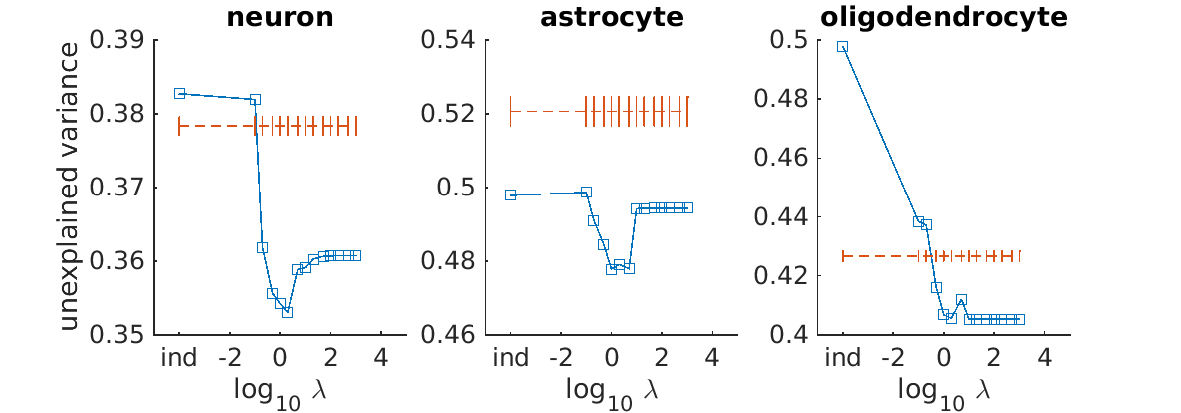
\includegraphics[width=0.99\textwidth]{3panels_var_AMY-CBC-DFC-HIP-V1C.png}
     \caption{Demixing RNA-seq data from 5 human brain regions \cite{brainspan}. Blue curve and squares correspond to the residual variance $(1-\rho^2)$ as a function of the strength of attractive region-to-region potentials $\lambda$. Red dashed line corresponds to a best-matched-sampels baseline (see text). At the optimum, the residual unexplained variance is reduced by 7\% for neurons, 8\% for astrocytes and 5\% in oligodendrocytes.}
    
\end{figure}


% [Add in the human experiment section We first verified that the brain regions in our data agree with the dev ontology: we clustered the brain regions in a hierarchical way and compared the resulting hierarchy to the dev ontology. We obtained very strong agreement …]. 




% ==========================================
\section{Summary and future directions}
We presented a probabilistic model for multi-region demixing approach aiming to estimate cell-type specific expression profiles from expression mixtures. We provide a simple and efficient way to solve it using repeated ANLS steps. We find that soft-sharing improves the accuracy of reconstruction as compared to demixing of individual regions, demixing of unified brain and random samples. This was consistent in both controlled samples where the ground truth was known and in postmortem human brains were we validated against mouse cell-type specific profiles.

The results shown above are expect to improve dramatically as further prior information is incorporated into the model. Some of that information is already available \cite{darmanis2015survey}, and we will add it in the near future.  Specifically, these include recent new measures of cell-type specific transcriptome from human cells, which can be used to determine the expected profiles $\mu_k$. Furthermore, estimates of coordinated expression among gene pairs can be used to determine the co-variation parameters in the model $\Sigma$.
As another direction, we expect that profiling might benefit from selecting subsets of genes that are strongly associated with specific cell types, and filtering genes that are not differentially expressed.

\newpage
\bibliography{nmf_multi}

\end{document}

